\chapter{Especificación de  Requisitos}
\section[Requisitos]{Requisitos}
En este apartado se resumirán los requisitos funcionales y no funcionales del proyecto, dividiéndolos en los requisitos de la interfaz de usuario y los requisitos internos de la aplicación.
\subsection[Requisitos interfaz]{Requisitos de la interfaz del usuario}
\subsubsection[Requisitos funcionales]{Requisitos funcionales}
\begin{itemize}
	\item \textbf{Mapa de la ciudad elegida por el usuario:} la aplicación mostrará el mapa de la ciudad seleccionada por el usuario, así como los alojamientos y puntos de interés que haya en la ciudad con marcadores en el mapa.
	\item\textbf{ Formulario de generación de rutas:} la aplicación dispondrá de una lista de puntos de interés y de alojamientos entre los que el usuario podrá elegir para generar la ruta. 
	\begin{itemize}
		\item Alojamiento: hostales y hoteles.
		\item Puntos de interés: museos, miradores, lugares históricos o de culto.
	\end{itemize}
	\item\textbf{ Especificación de las rutas:} la aplicación deberá mostrar los puntos de interés que contiene la ruta como marcadores, así como las direcciones que deberá seguir el usuario para llegar desde un punto hasta otro. También mostrará una lista ordenada de dichos puntos en los cuales se especificará la hora de entrada y salida aproximadas de cada punto de interés.
	\item \textbf{Información sobre los marcadores:} la aplicación deberá mostrar información referente a los marcadores mostrados en la interfaz. Dicha información será el nombre de dicho punto de interés.
\end{itemize}
\subsubsection[Requisitos no funcionales]{Requisitos no funcionales}
\begin{itemize}
	\item \textbf{Interfaz:} la interfaz deberá ser atractiva, ligera y lo más intuitiva posible.
	\item \textbf{Plataforma:} la aplicación estará disponible para todos los dispositivos móviles que utilicen el sistema operativo Android a partir de la versión 5.0 (Lollipop).
\end{itemize}

\subsection[Requisitos internos]{Requisitos de la aplicación}
\subsubsection[Requisitos funcionales]{Requisitos funcionales}
\begin{itemize}
	\item \textbf{Recepción de peticiones del cliente:} la aplicación será capaz de recibir peticiones que el cliente le envía a través de la interfaz gráfica que contienen los puntos de interés seleccionados por el usuario.
	\item \textbf{Cálculo y retorno de rutas óptima:} a partir de los datos proporcionados por el usuario y la información que se tiene sobre dichos datos; la aplicación calculará y devolverá la ruta que después será mostrada en la interfaz.
	\item \textbf{Publicación de lista de alojamientos y puntos de interés:} la aplicación tendrá acceso a una lista de alojamientos y puntos de interés que el usuario podrá seleccionar desde la interfaz de la aplicación.
	\item \textbf{Publicación de la ruta en una mapa:} la aplicación será capaz de mostrar en la interfaz de usuario los puntos de interés seleccionados en un mapa, así como una lista ordenada de la ruta y el camino para llegar desde un punto de interés hasta el siguiente. El primer punto siempre será el alojamiento seleccionado por el usuario.
\end{itemize}
\subsubsection[Requisitos no funcionales]{Requisitos no funcionales}
\begin{itemize}
	\item \textbf{Envío de peticiones de puntos de interés y alojamientos:} la aplicación deberá mandar peticiones a un servidor que es capaz de conectarse a una base de datos para obtener los datos necesarios sobre alojamientos y puntos de interés. Dicha información se devuelve en un fichero .json.
	\item \textbf{Importación de información sobre puntos de interés y alojamientos:} tras obtener los puntos de interés y alojamientos del servidor; la aplicación deberá procesar la información contenida en el fichero .json para mostrarlos en la interfaz.
	\item \textbf{Envío de peticiones a servidor de cálculo de matrices de tiempos:} la aplicación deberá mandar peticiones a un servidor que calculará la distancias entre los puntos seleccionados por el usuario. Dichos tiempos se devuelve en un archivo .json.
	\item \textbf{Importación de matriz de tiempos:} una vez se ha obtenido el archivo .json que contiene la matriz de tiempos, la aplicación debe procesar dicho fichero y guardar la matriz para su uso en el cálculo de rutas.
	\item \textbf{Envío de peticiones para obtener ruta entre los distintos puntos de interés que contiene la solución calculada:} la aplicación deberá enviar peticiones a un servidor que devolverá la ruta a seguir el usuario para llegar a cada uno de los puntos de interés. Dicha información se devuelve en un archivo .json.ç
	
	\item \textbf{Importación de direcciones entre puntos de interés:} la aplicación deberá guardar y procesar la información que contiene el archivo .json para después mostrar las direcciones en la interfaz de usuario.
\end{itemize}

\section[Casos de uso]{Diagramas de casos de uso}
\subsection[Interfaz de usuario]{Interfaz de usuario}
\begin{figure}[H]
	\centering
	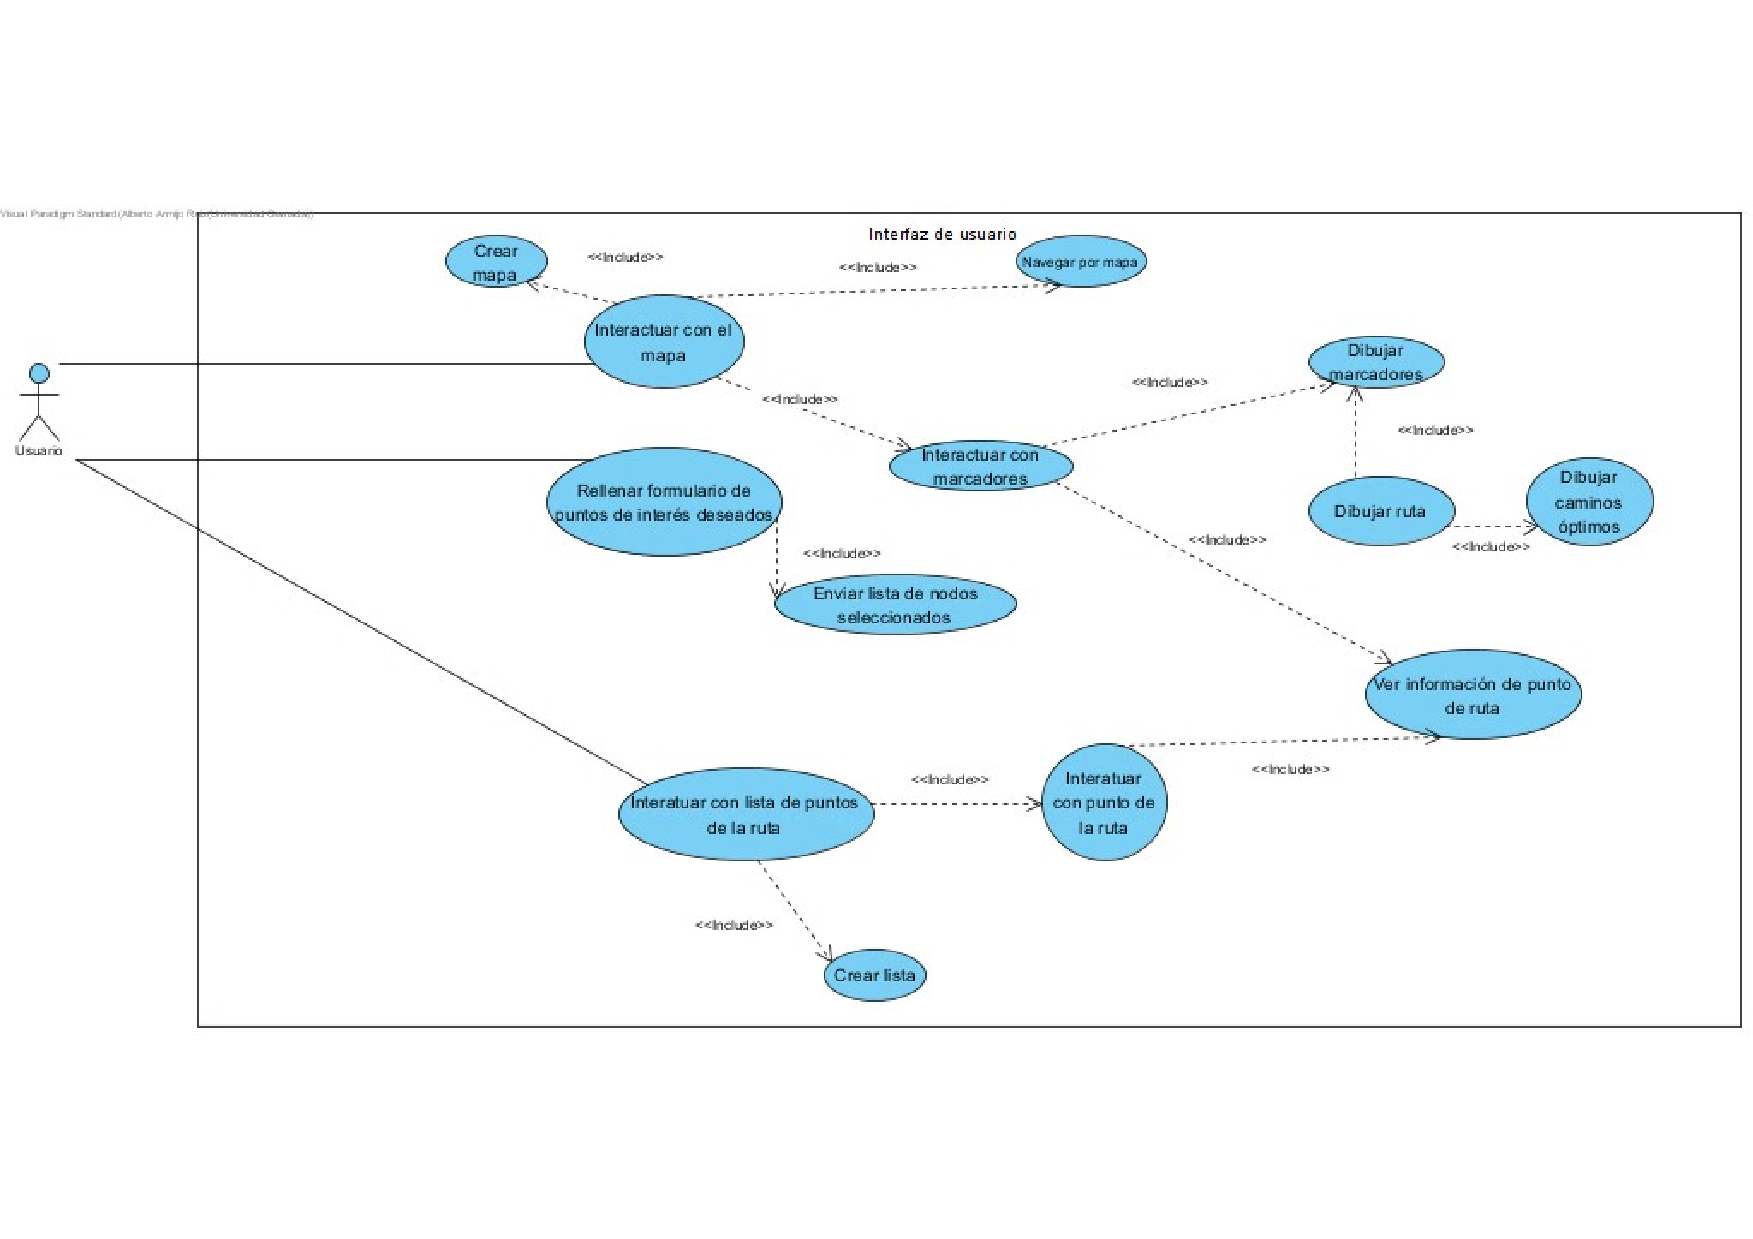
\includegraphics[scale=0.5]{imagenes/Interfaz.pdf}
	\caption{Diagrama de casos de uso de la interfaz de usuario}
	\label{fig:user_interface}
\end{figure}

\subsection[Aplicación]{Aplicación móvil}
\begin{figure}[H]
	\centering
	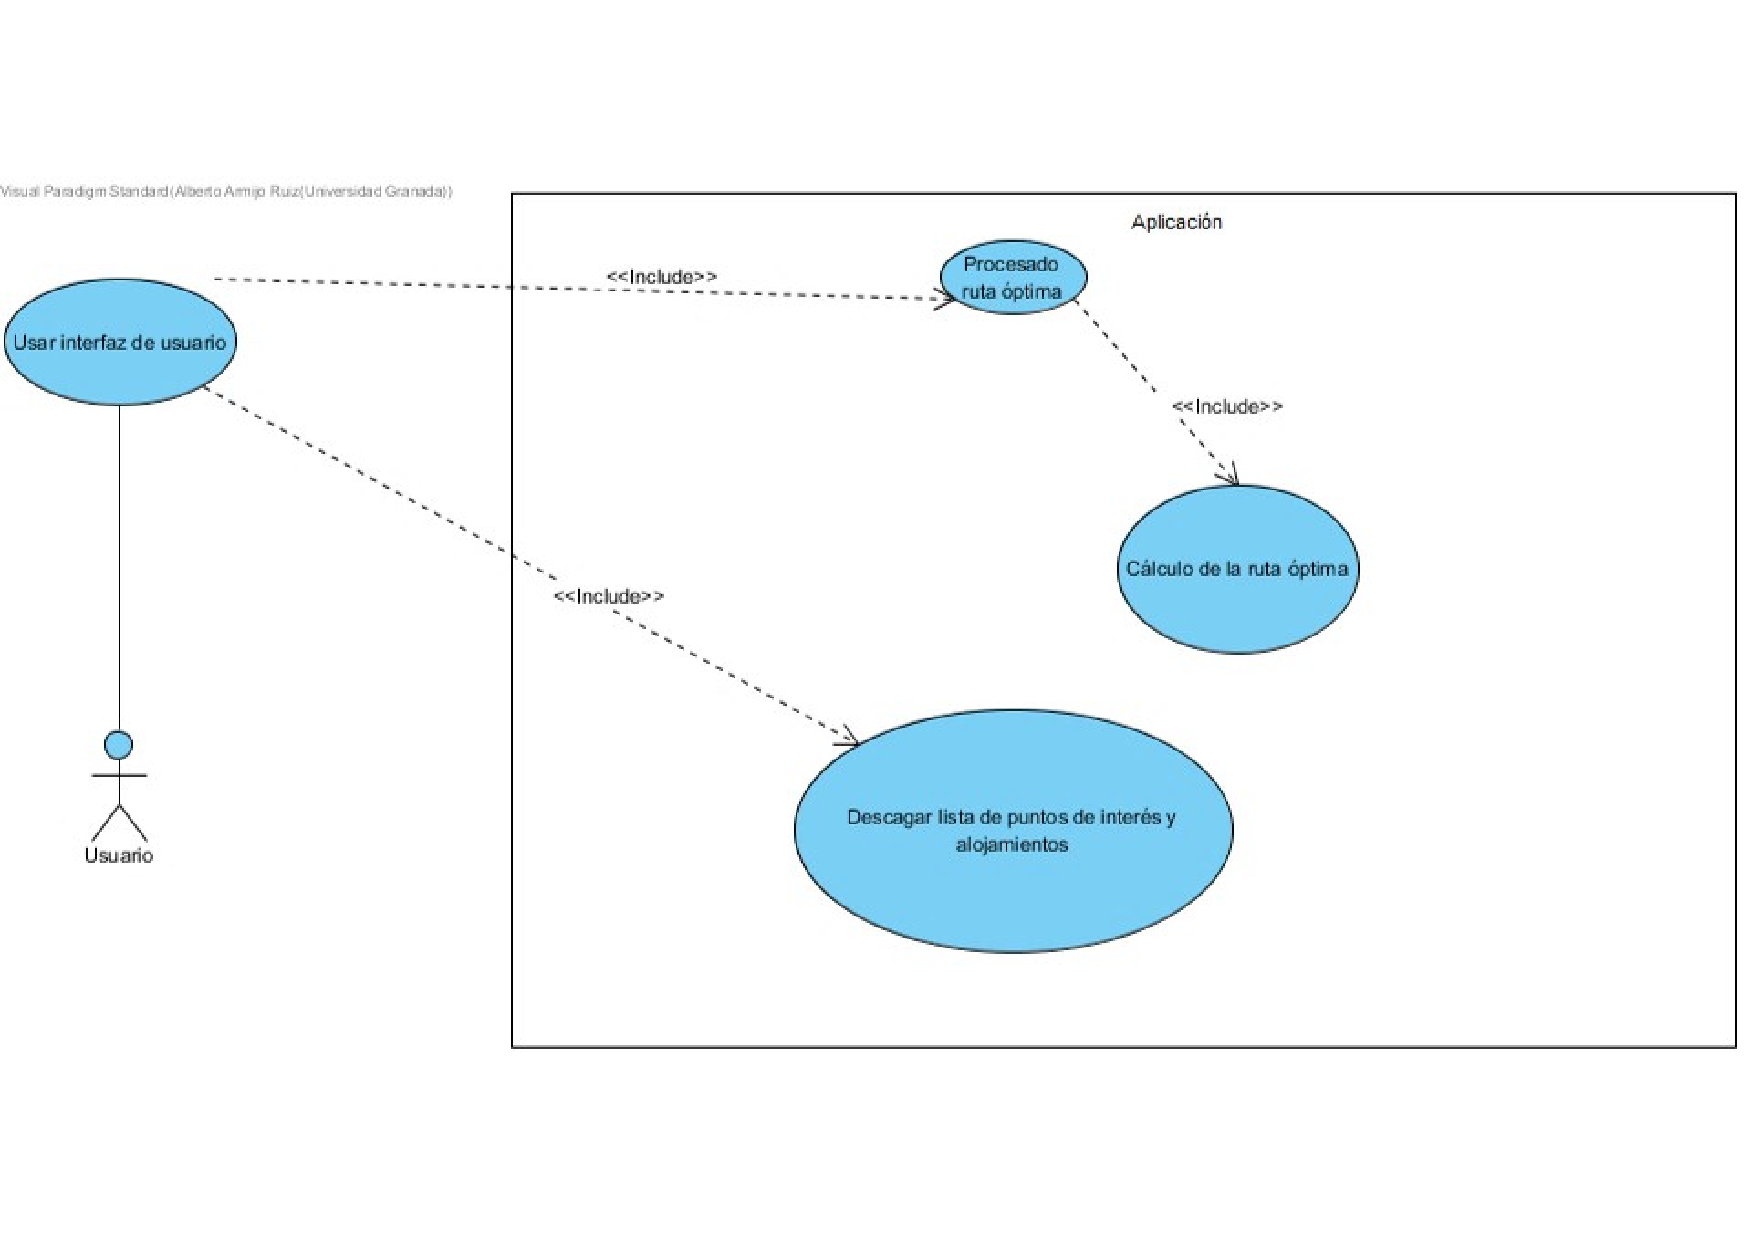
\includegraphics[scale=0.55]{imagenes/Aplicacion.pdf}
	\caption{Diagrama de casos de uso de la aplicación}
	\label{fig:app}
\end{figure}

\section[Fuente de los datos]{Fuente de los datos}
\subsection[OSM]{Open Street Map}
Ya que el objetivo de la aplicación fue crear rutas a partir de puntos de interés, se requirió obtener una lista con todos los puntos de interés y alojamientos disponibles en una ciudad con la suficiente información para que puedan ser usados para calcular rutas.\newline
Tras investigar diferentes posibilidades, se decidió utilizar OpenStreetMap, el cual es un proyecto colaborativo que permite crear mapas y editar los ya existentes.\newline
\begin{figure}[H]
	\centering
	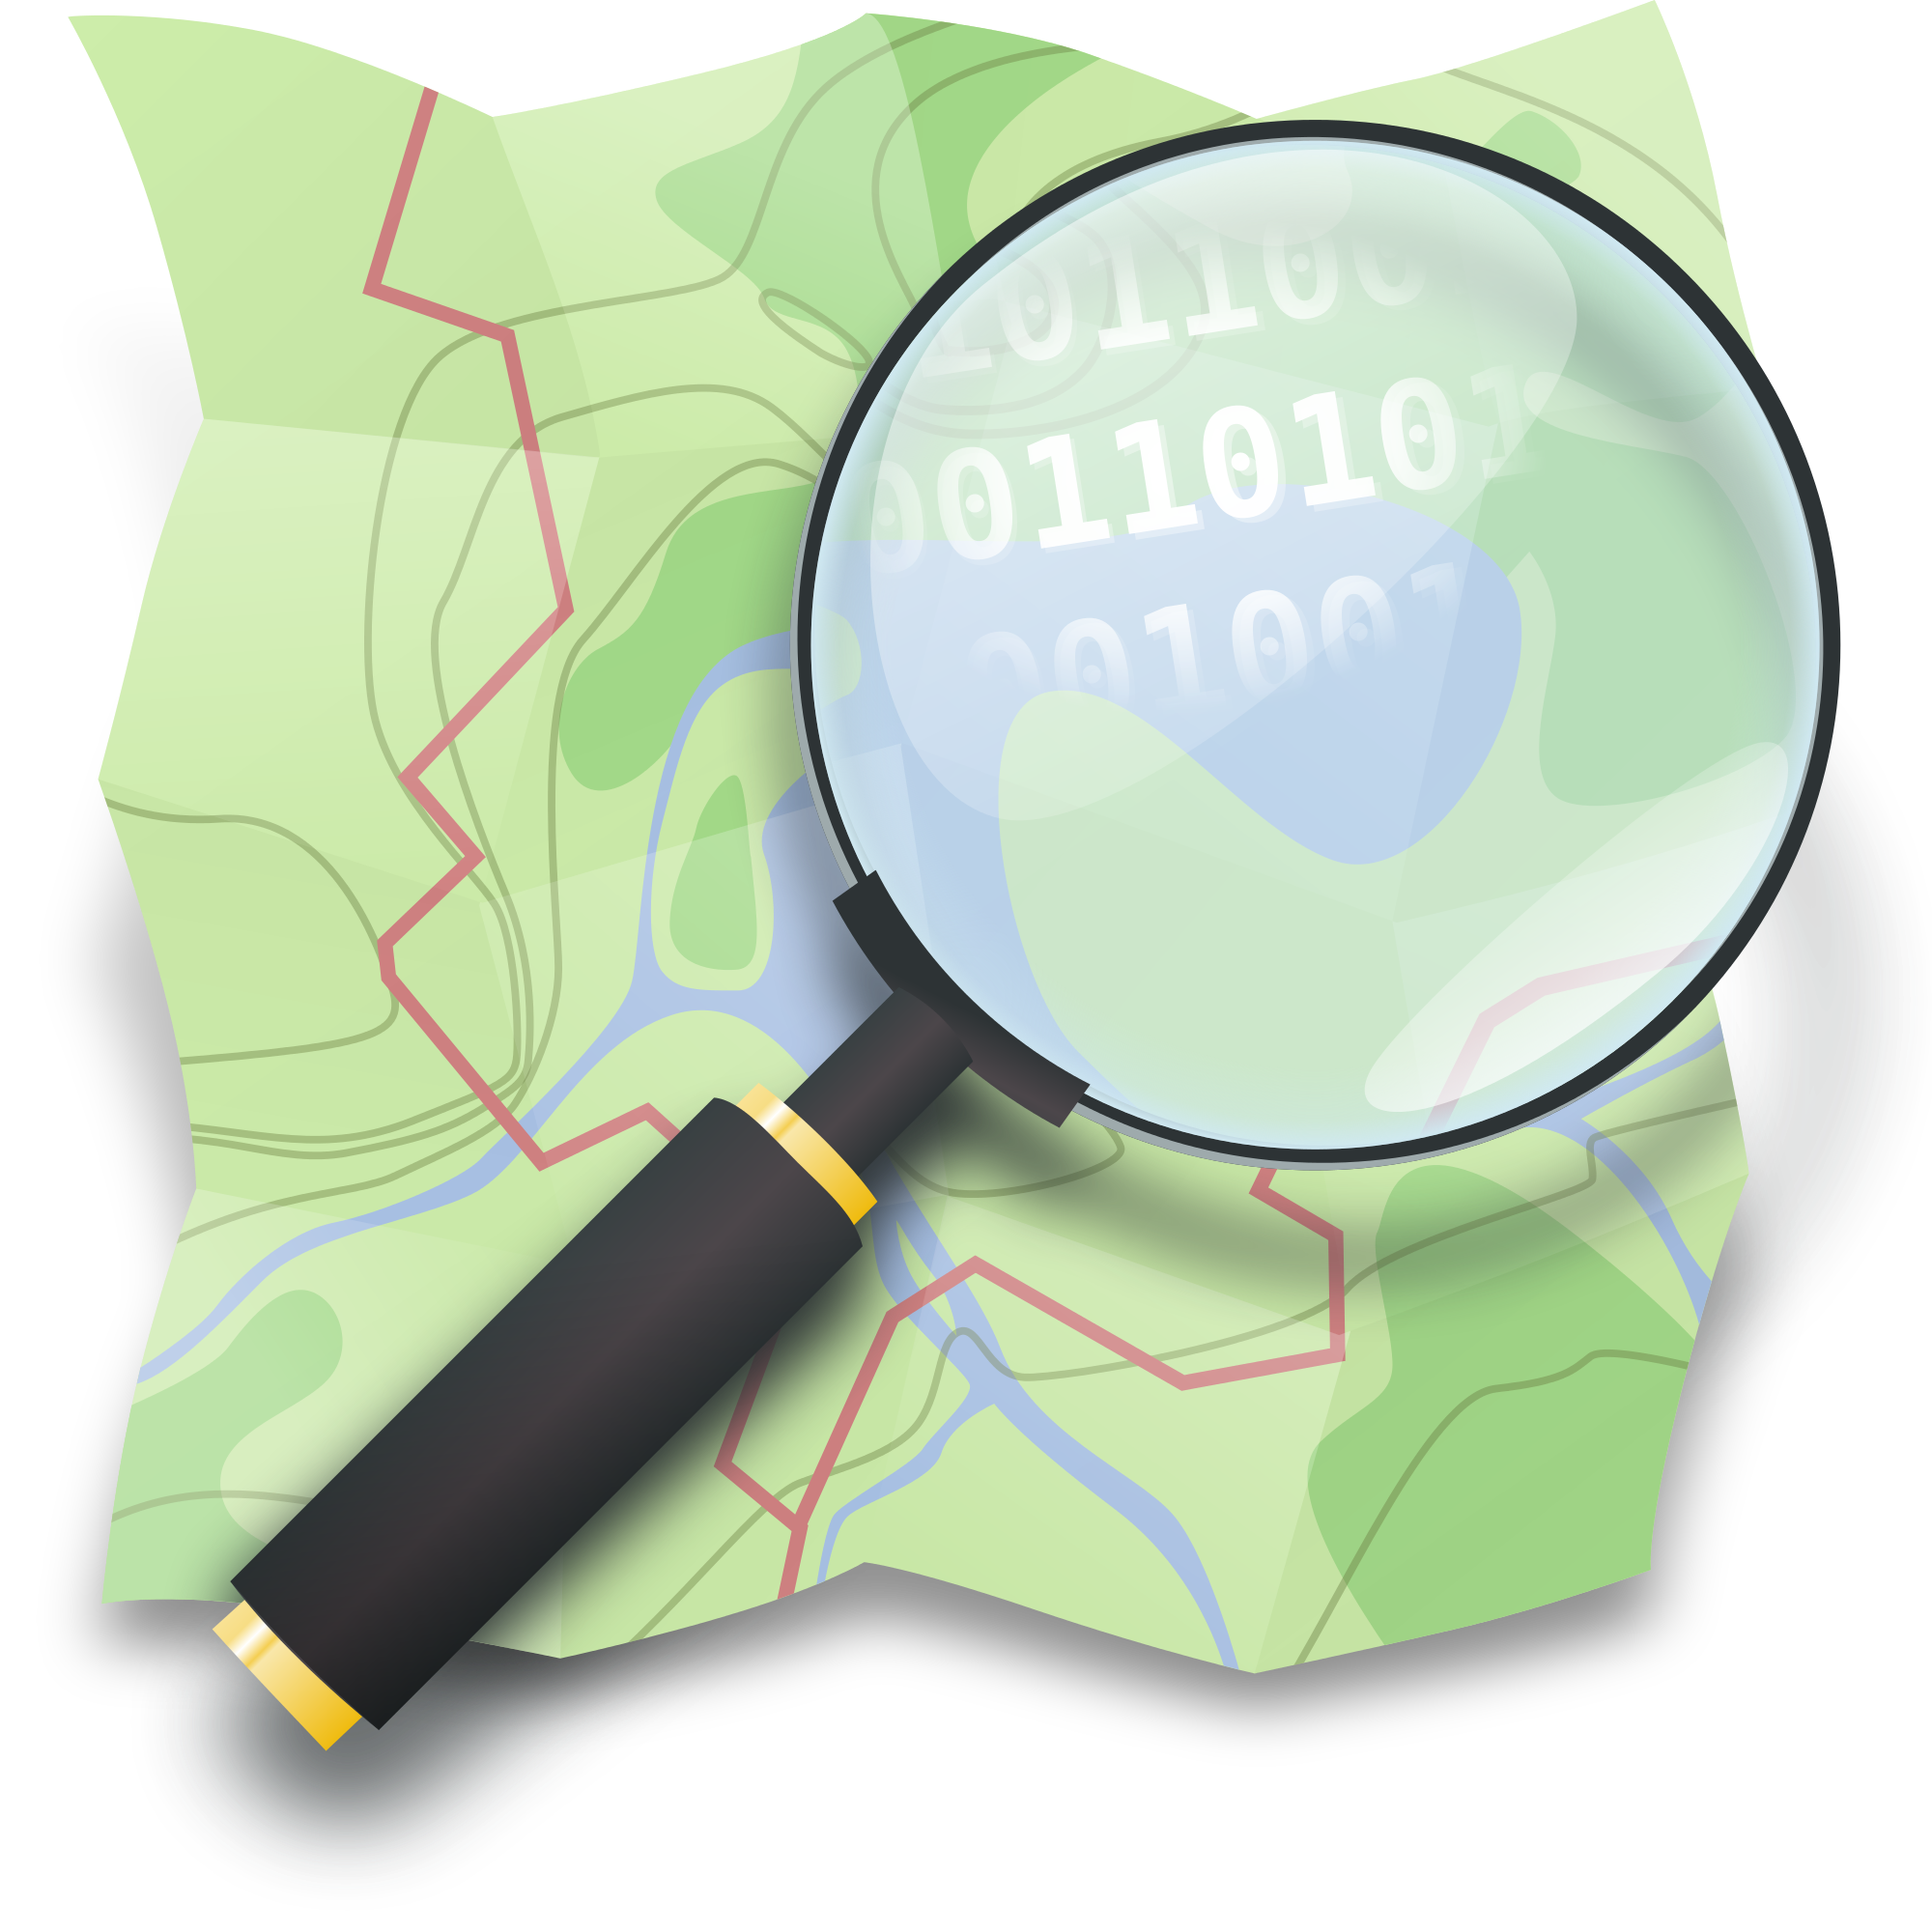
\includegraphics[scale=0.05]{imagenes/Openstreetmap_logo}
	\caption{Logo de OpenStreetMap}
	\label{fig:openstreetmap}
\end{figure}
OpenStreetMap tiene una web \cite{openstreetmap} en la cual puedes editar cualquiera de los puntos de interés que contiene el mapa o crear nuevos siempre que estés registrado. Además, cuenta con diferentes tipos de estructuras para representar edificios, carreteras, etc... OpenStreetMap utiliza tres tipos diferentes de información:\newline
\begin{itemize}
	\item Líneas: sirven para describir cualquier tipo de vía, como por ejemplo carreteras.
	\item Nodos: sirven para definir cualquier tipo de edificio, como por ejemplo farmacias o museos.
	\item Áreas: sirven para definir el espacio ocupado por un nodo, por ejemplo, un parque. Dichas áreas están formadas un conjunto de nodos que delimitan el área.
\end{itemize}
Al no estar disponible el acceso a la base de datos que contiene OpenStreetMap de forma directa se tuvo que buscar una API para poder obtener los datos.
\subsection[Overpass]{Overpass API}
Para obtener la información necesaria de OpenStreetMap, se necesitó buscar una API que permitiera obtener dicha información. Overpass es una API que permite hacer consultas sobre puntos de interés y que utiliza la información de OpenStreetMap para devolver la información sobre los puntos de interés. Dichas consultas pueden realizarse mediante urls. Las respuestas obtenidas por Overpass se devuelven en formato JSON, dentro de dicho fichero se encuentra un array llamado \enquote{elements} que contiene cada uno de los elementos. A continuación, se muestra una parte del fichero que devuelve Overpass para alojamientos y puntos de interés en Granada.\newline
\begin{lstlisting}[caption=Respuesta Overpass sobre alojamientos y puntos de interés en Granada]
{
"version": 0.6,
"generator": "Overpass API 0.7.54.13 ff15392f",
"osm3s": {
"timestamp_osm_base": "2018-02-27T10:23:02Z",
"copyright": "The data included in this document is from www.openstreetmap.org. The data is made available under ODbL."
},
"elements": [

{
"type": "node",
"id": 533647928,
"lat": 37.1734517,
"lon": -3.5888790,
"tags": {
"name": "Museo Manuel de Falla",
"tourism": "museum"
}
},
{
"type": "node",
"id": 940435771,
"lat": 37.1770011,
"lon": -3.5900734,
"tags": {
"name": "Museo de la Alhambra",
"tourism": "museum"
}
},
},
{
"type": "node",
"id": 1351215450,
"lat": 37.1765624,
"lon": -3.5897641,
"tags": {
"designation": "Museo de Bellas Artes",
"email": "museobellasartesgranada.ccul@juntadeandalucia.es",
"name": "Museo de Bellas Artes",
"tourism": "museum"
}
},
{
"type": "node",
"id": 1667155336,
"lat": 37.1625928,
"lon": -3.6066354,
"tags": {
"name": "Parque de las Ciencias",
"tourism": "museum"
}
},
...
{
"type": "node",
"id": 4029579625,
"lat": 37.1800207,
"lon": -3.5957336,
"tags": {
"addr:city": "Granada",
"addr:housenumber": "18",
"addr:postcode": "18010",
"name": "Makuto Guesthouse",
"tourism": "hostel",
"website": "http://makutohostel.com"
}
},
]
}
\end{lstlisting}

Para generar dicho fichero de salida, se deben ajustar ciertos parámetros dentro de la petición que se hace a Overpass. Para probar diferentes parámetros, se puede utilizar la herramienta de Overpass llamada Overpass-turbo.\newline
Overpass-turbo es una página web que contiene un mapa interactivo y una ventana donde nos permite escribir consultas a Overpass; desde ahí, se puede generar un script que encuentre todos los puntos de interés y alojamientos en una ciudad; después, dicho script puede exportarse como una petición en formato URL para utilizarla sin necesidad de utilizar Overpass-turbo. Dentro de dicho script debe especificarse los tipos de nodos que se quieren obtener, la información sobre los diferentes tipos de nodos se encuentra dentro de la documentación de OpenStreetMap \cite{openstreetmap_doc}.El script para obtener la información mostrada arriba es el siguiente. \newline
\begin{lstlisting}[caption=Script para encontrar todos los puntos de interés y alojamientos de una ciudad]
[out:json][timeout:100]; 

(node["place"="city"]["name"="Granada"]["is_in:province"="Granada"]["is_in:country"="Spain"];)->.ciudad; 

node["tourism"="museum"](around.ciudad:7000);
out;>;out;

node["tourism"="viewpoint"](around.ciudad:7000);
out;

// Catedrales.
node["building"="cathedral"](around.ciudad:7000);
out;

// Hoteles.
node["tourism"="hotel"](around.ciudad:7000);
out;

// Hotales.
node["tourism"="hostel"](around.ciudad:7000);
out;
\end{lstlisting}

\subsection[OSRM]{Open Source Routing Machine}
Como la aplicación necesita obtener la matriz de distancias entre los distintos puntos seleccionados por el usuario, se investigó para encontrar una herramienta que permitiera obtener dicha matriz a través de peticiones mediante URL.\newline
Tras probar con varias herramientas, se optó por usar OSRM \cite{osmr},la cual es de uso gratuito. OSRM permite hacer peticiones a sus servidores\cite{osmr_doc} o montar uno propio \cite{osmr_backend}.\newline
OSRM devuelve de sus peticiones un archivo JSON que contiene las distancias entre los puntos especificados en la petición, el tiempo que se tarda en llegar desde un punto a otro está guardado en un array llamado \enquote{durations}; cada elemento de dicho array contiene otro array con los tiempos desde dicho punto de interés al resto de puntos de interés. Un ejemplo de la salida de OSRM es el siguiente:
\begin{lstlisting}[caption=Salida de OSRM]
{"durations":
	[[0,245,165.9,165.9,165.9,44.9,162.3,130.6,130.6,44.9,56.2],
	[245,0,79.1,79.1,79.1,200.1,82.7,114.4,114.4,200.1,188.8],
	[165.9,79.1,0,0,0,121,3.6,35.3,35.3,121,109.7],
	[165.9,79.1,0,0,0,121,3.6,35.3,35.3,121,109.7],
	[165.9,79.1,0,0,0,121,3.6,35.3,35.3,121,109.7],
	[44.9,200.1,121,121,121,0,117.4,85.7,85.7,0,11.3],
	[162.3,82.7,3.6,3.6,3.6,117.4,0,31.7,31.7,117.4,106.1],
	[130.6,114.4,35.3,35.3,35.3,85.7,31.7,0,0,85.7,74.4],
	[130.6,114.4,35.3,35.3,35.3,85.7,31.7,0,0,85.7,74.4],
	[44.9,200.1,121,121,121,0,117.4,85.7,85.7,0,11.3],
	[56.2,188.8,109.7,109.7,109.7,11.3,106.1,74.4,74.4,11.3,0]],
	...
}
\end{lstlisting}

\subsection[Google Routes API]{Google Maps Directions API}
Dado que la aplicación debe mostrar el camino óptimo entre dos puntos seleccionados en la solución, se buscó una herramienta que lo calculara. Tras investigar y probar diferentes herramientas, se optó por utilizar Google Maps Directions API \cite{directions_api}.\newline
Esta herramienta permite hacer peticiones a un servidor y devuelve un archivo JSON que contiene la ruta que se debe seguir. Este archivo se debe procesar para obtener las polilíneas que represetan el camino entre dos puntos. Un ejemplo de este archivo es el siguiente.\newline
\begin{lstlisting}[caption=Salida de Google Maps Directions API]
{"routes" : [
...
"legs" : [
{
"distance" : {
"text" : "2.0 km",
"value" : 2044
},
"duration" : {
"text" : "25 min",
"value" : 1496
},
"end_location" : {
"lat" : 37.1622873,
"lng" : -3.6068922
},
"start_location" : {
"lat" : 37.1761203,
"lng" : -3.6025799
},
"steps" : [
{
"distance" : {
"text" : "0.1 km",
"value" : 115
},
"duration" : {
"text" : "1 min",
"value" : 75
},
"end_location" : {
"lat" : 37.1757377,
"lng" : -3.6037831
},

"polyline" : {
"points" : "w}{aFbs~TNx@VrAV|@Jb@"
},
"start_location" : {
"lat" : 37.1761203,
"lng" : -3.6025799
},
"travel_mode" : "WALKING"
},
{
"distance" : {
"text" : "0.4 km",
"value" : 354
},
"duration" : {
"text" : "4 min",
"value" : 252
},
"end_location" : {
"lat" : 37.1738268,
"lng" : -3.6069271
},

"polyline" : {
"points" : "k{{aFrz~T@Hp@nBP`@T\\j@p@fA|ADF~AtBfAlD"
},
"start_location" : {
"lat" : 37.1757377,
"lng" : -3.6037831
},
"travel_mode" : "WALKING"
},
}
\end{lstlisting}